\documentclass[12pt,a4paper,oneside]{article}
\usepackage[colorlinks=true]{hyperref}
\usepackage[utf8]{inputenc}
\usepackage[czech]{babel}
\usepackage{pdfpages}
\usepackage{graphicx}
\textwidth 16cm \textheight 25cm
\topmargin -1.3cm 
\oddsidemargin 0cm
\usepackage{footnote}
\pagestyle{empty}
\begin{document}
\title{Modul převodníku TTL na CAN - TTLCAN01B}
\author{Jakub Kákona, kaklik@mlab.cz}
\maketitle

\thispagestyle{empty}
\begin{abstract}
Modul je určen pro připojení procesorových modulů na fyzickou vrstvu sběrnice CAN.
\end{abstract}

\begin{figure} [htbp]
\begin{center}
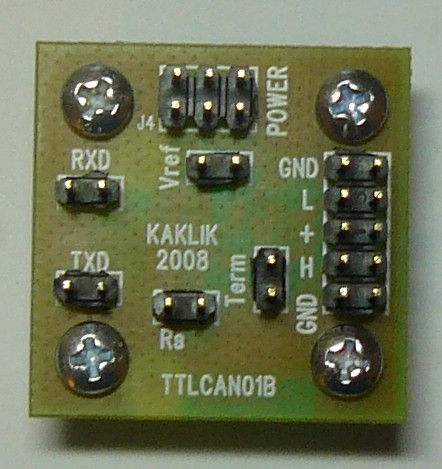
\includegraphics [width=80mm] {./img/TTLCAN01B_Top_Big.JPG} 
\end{center}
\end{figure}

\begin{figure} [b]

\includegraphics [width=25mm] {./img/TTLCAN01B_QRcode.png} 
\end{figure}

\newpage
\tableofcontents


\section{Technické parametry}
\begin{table}[htbp]
\begin{center}
\begin{tabular}{|c|c|c|}
\hline
\multicolumn{1}{|c|}{Parametr} & \multicolumn{1}{|c|}{Hodnota} & \multicolumn{1}{|c|}{Poznámka} \\ \hline
Napájecí napětí & +5V &  30 mA \\ \hline
Pracovní napětí  vstupů & do $\pm$ 5V &  \\ \hline
Maximální budící proud výstupů & max 60 mA & \\ \hline
\end{tabular}
\end{center}
\end{table}

\newpage
\section{Popis konstrukce}

\subsection{Zapojení}
Modul obsahuje základní ochranu proti přepěťovým špičkám a terminační rezistor který lze juperem odpojit, což je vhodné u modulů, které jsou zapojeny uprostřed sběrnice.  Datové vývody  jsou vyvedeny na hřebínky ve standardní konfiguraci MLAB, která je vhodná pro kratší mezimodulové spoje. V případě potřeby použití modulu na delší spoj (desítky metrů) je vhodné k modulu přidat ochranné transily pro zvýšení odolnosti proti přepětí. To lze udělat připojením konverzního modulu s konektorem RJ45. Pak lze použít standardní UTP patch kabely, které jsou vhodné pro vedení na delší vzdálenosti.   

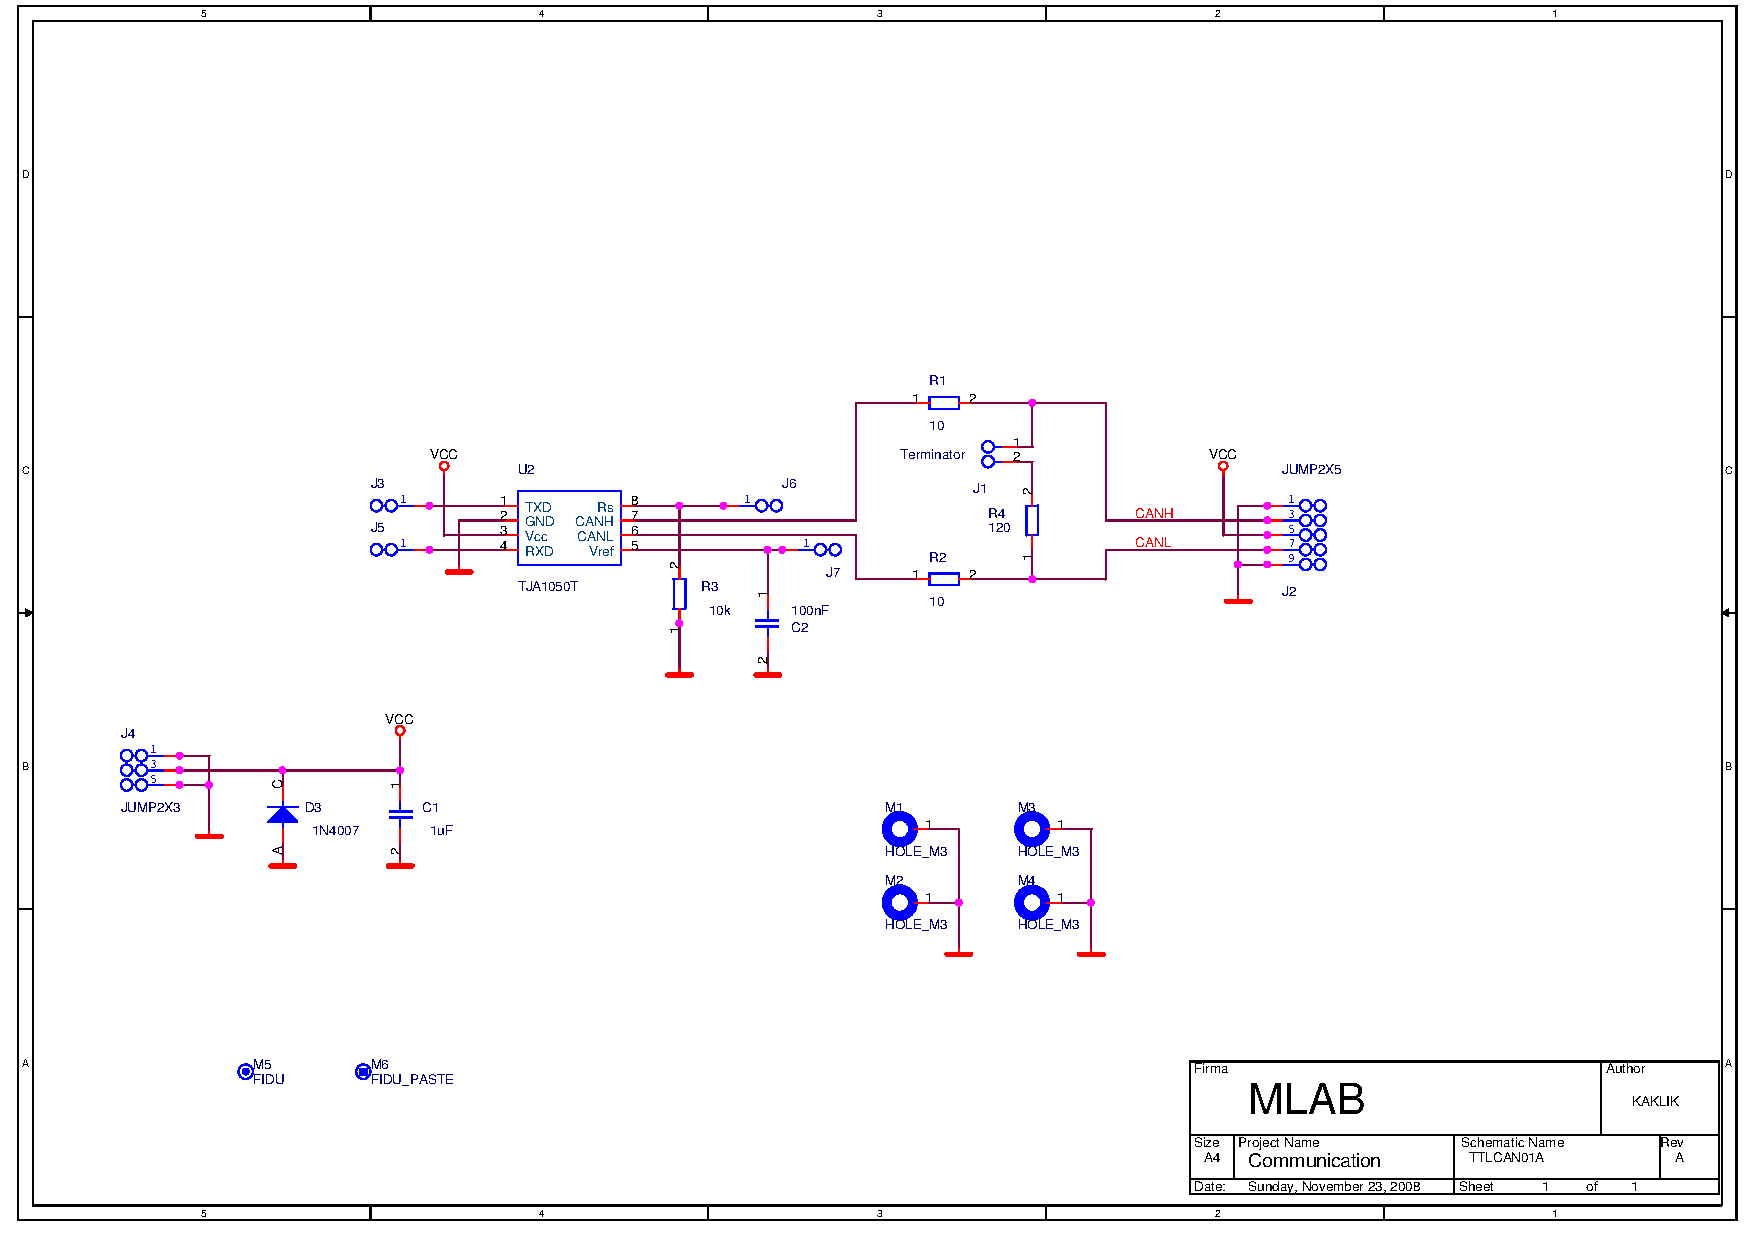
\includepdf[pages={1},landscape=true]{../../SCH/TTLCAN01B.pdf}

\subsection{Odrušení}

Vyzařování je v případě modulu značně potlačeno  differenční fyzickou vrstvou sběrnice.  K její správné funkci je ale potřeba využívat kroucených párů.  Pro vedení signálů CAN jsou proto vhodné například UTP kabely. Kde signály CAN jsou vedeny po jednom differenčním páru.   

\section{Výroba a testování}

Modul se testuje optickou kontrolou spojů a následným připojením na laboratorní zdroj s omezením proudu. Dále by po připojení dvou modulů k USBRS23201B a nastavení jednoho modulu na příjem a druhý na vysílání mělo být možné posílat znaky. Podrobněji je tento testovací postup popsán na wiki \cite{wiki-TTLCAN}.


\subsection{Osazení}

Modul se osazuje standardním způsobem požívaným pro SMD součástky. 

\begin{figure} [h!tbp]
  \centering
  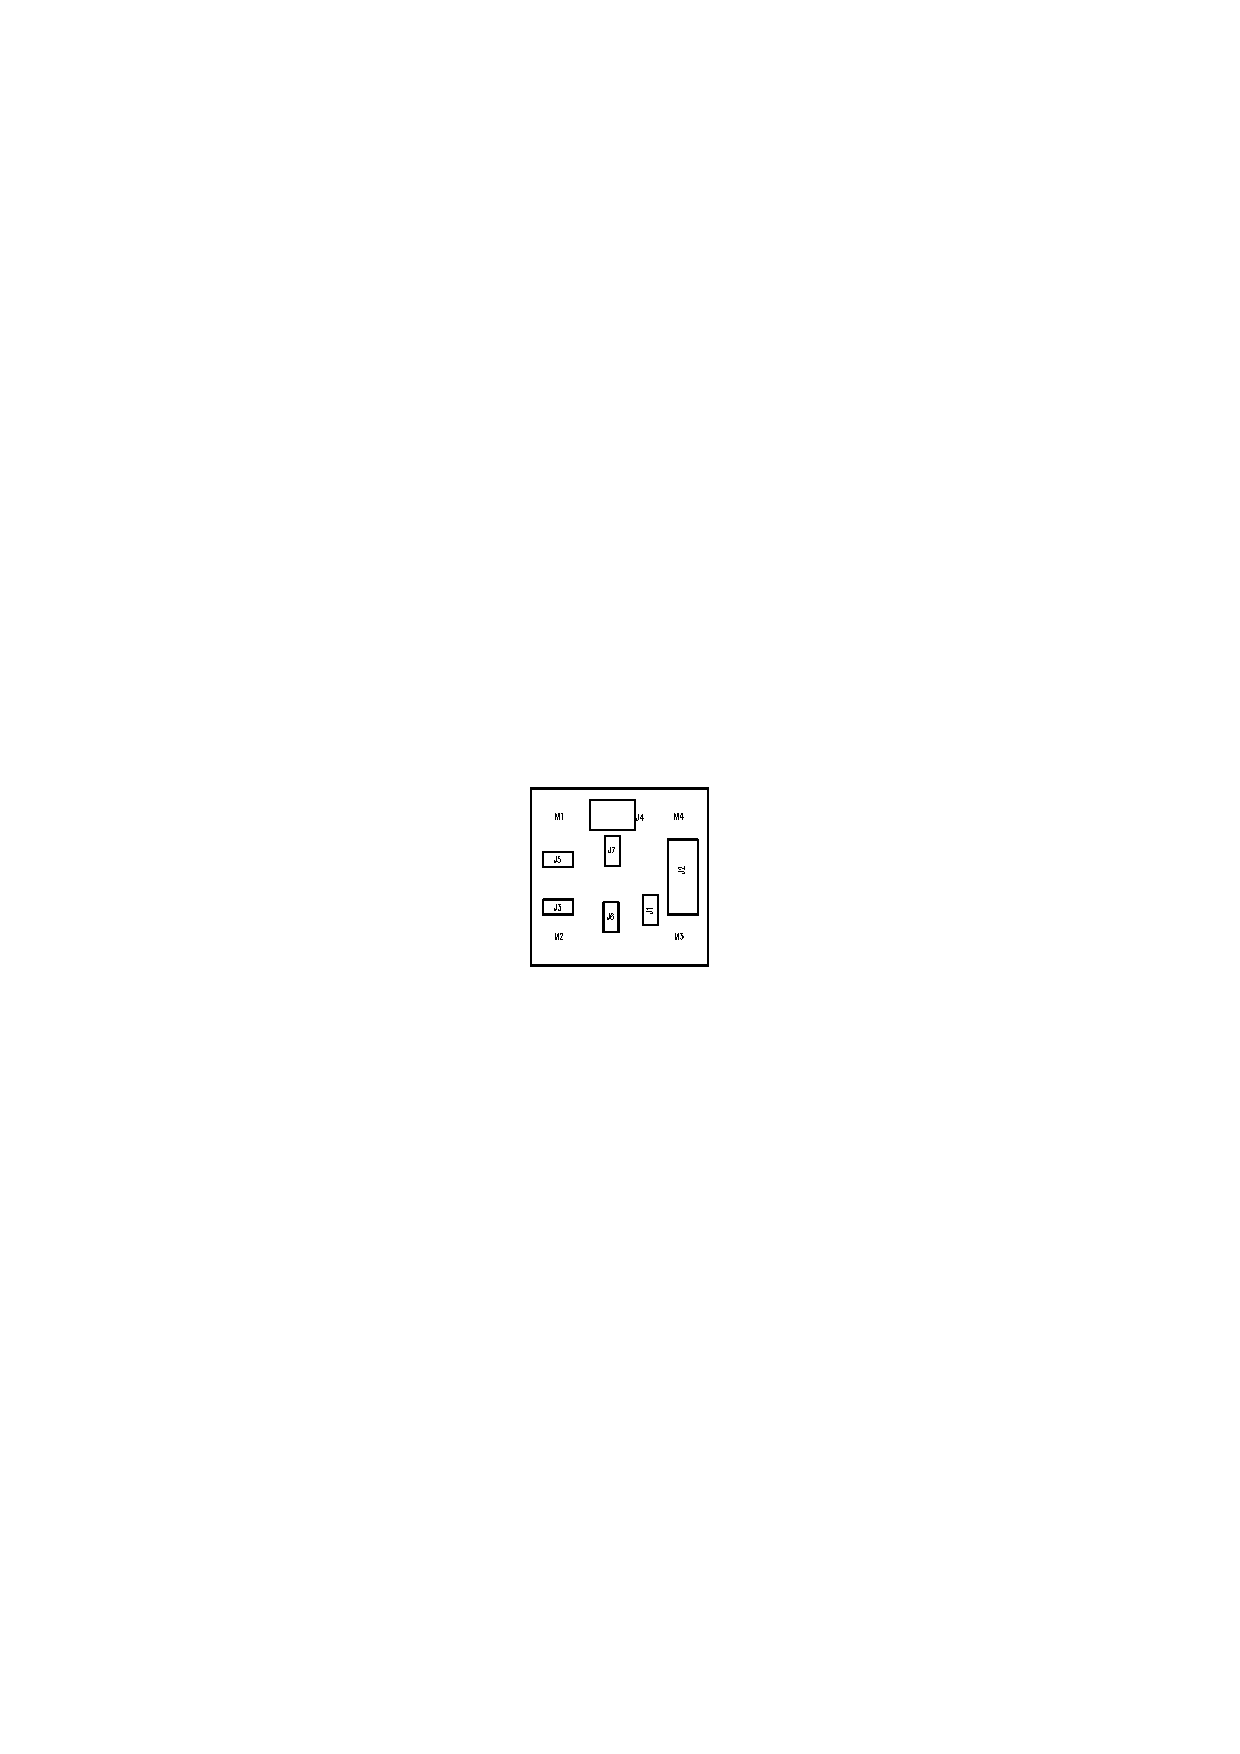
\includegraphics[trim = 8.5cm 13.0cm 8.5cm 13.0cm, clip, width=6.5cm]{../../CAM_DOC/O1.pdf}
  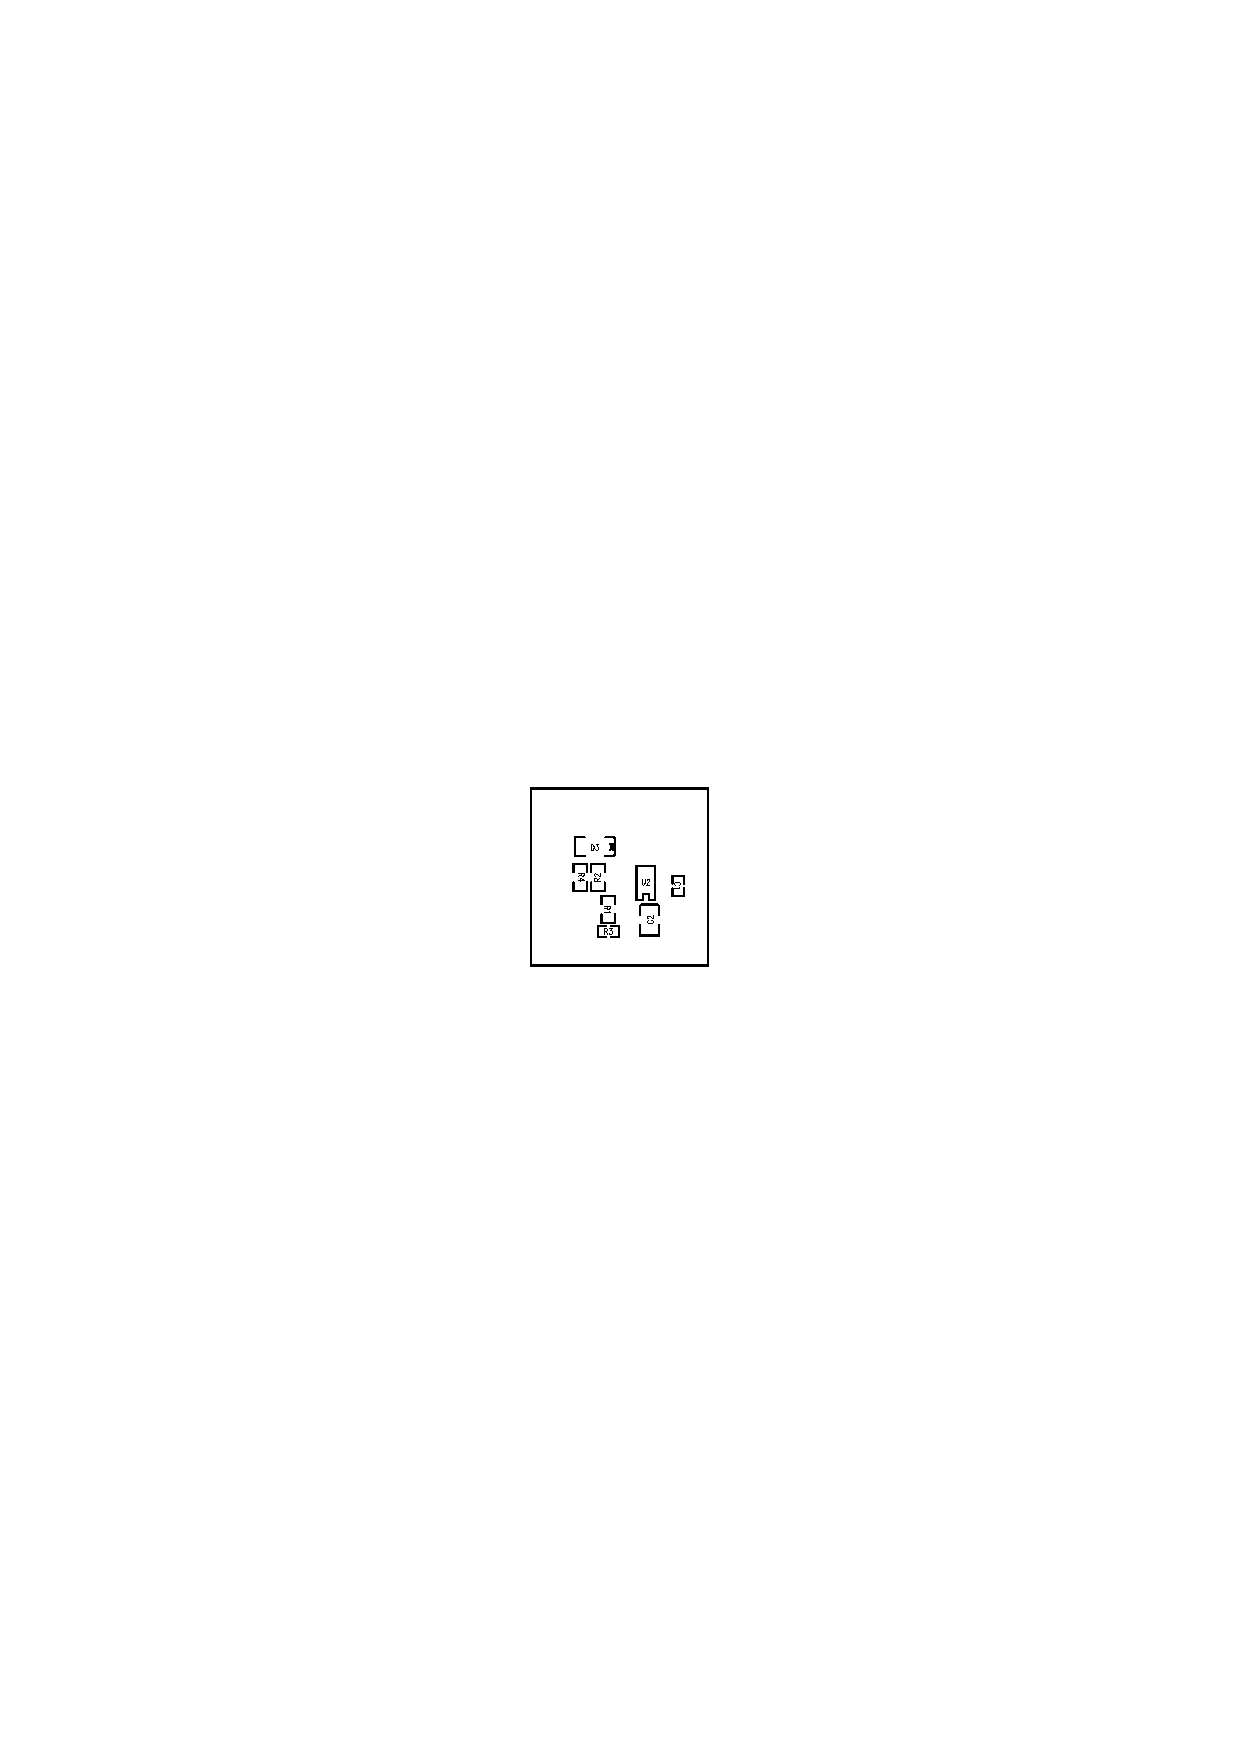
\includegraphics[trim = 8.5cm 13.0cm 8.5cm 13.0cm, clip, width=6.5cm]{../../CAM_DOC/O2.pdf}
  \caption{Osazovací plán horní a spodní strany plošného spoje}
  \label{fig:osazovaci_plan}
\end{figure}

\begin{savenotes}
\begin{table}[h!]
\begin{center}
\begin{tabular}{ |c|c|c|c| }
\hline 
Počet & Označení & Typ  & Pouzdro  \\ 
\hline 
1	&	C1	&	C0805	&	1uF	\\
1	&	C2	&	C0805	&	100nF	\\
1	&	D3	&	SMA	&	M4 \\
1	&	J1	&	JUMP2	&	Terminator	\\
1	&	J2	&	JUMP2X5	&	JUMP2X5	\\
4	&	J3,J5,J6,J7	&	JUMP2X1	&	JUMP2X1	\\
1	&	J4	&	JUMP2X3	&	JUMP2X3	\\
2	&	R1,R2	&	R1206	&	10	\\
1	&	R3	&	R0805	&	10k	\\
1	&	R4	&	R1206	&	120	\\
1	&	U2	&	SO8\_150	&	TJA1050T	\\
\hline 
\end{tabular}
\end{center}
\caption{Seznam součástek osazovaných na desku plošného spoje.}
\label{seznam_soucastek_galvanic_isolation}
\end{table}
\end{savenotes}



\section{Programové vybavení}

Samotný modul pro svoje fungování nepotřebuje speciální firmware. Lze jej provozovat i na jiných protokolech, než CAN. Modul pouze vytváří fyzickou vrstvu této sběrnice.

\begin{thebibliography}{99}
\bibitem{wiki-TTLCAN}{TTLCAN MLAB wiki} 
\href{http://wiki.mlab.cz/doku.php?id=cs:ttlcan}{Převodník úrovní TTL a CAN TTLCAN01B}

\end{thebibliography}
\end{document}